\section{Velocity Controller}\label{sec:velocityController}
The purpose of the velocity controller is to preserve the vehicle at a steady velocity, when going uphill, downhill and when turning, this is in conjunction with the velocity requirement from \secref{sec:Requirements}. The three most widely utilized controllers are the proportional, integral and differential controllers \todo{Source}. Usually all three controllers combined are not required when controlling a system. Different controller approaches are explored in the following segment, starting with the controller which is the most frequently utilized controller, alone or in combination with others, the proportional controller.

\subsection{P-Controller}
As illustrated on \figref{proportionalController} the P-controller, \si{K_p}, is a proportional gain which is multiplied with the direct term.
%
\begin{figure}[H]
 	\centering
 	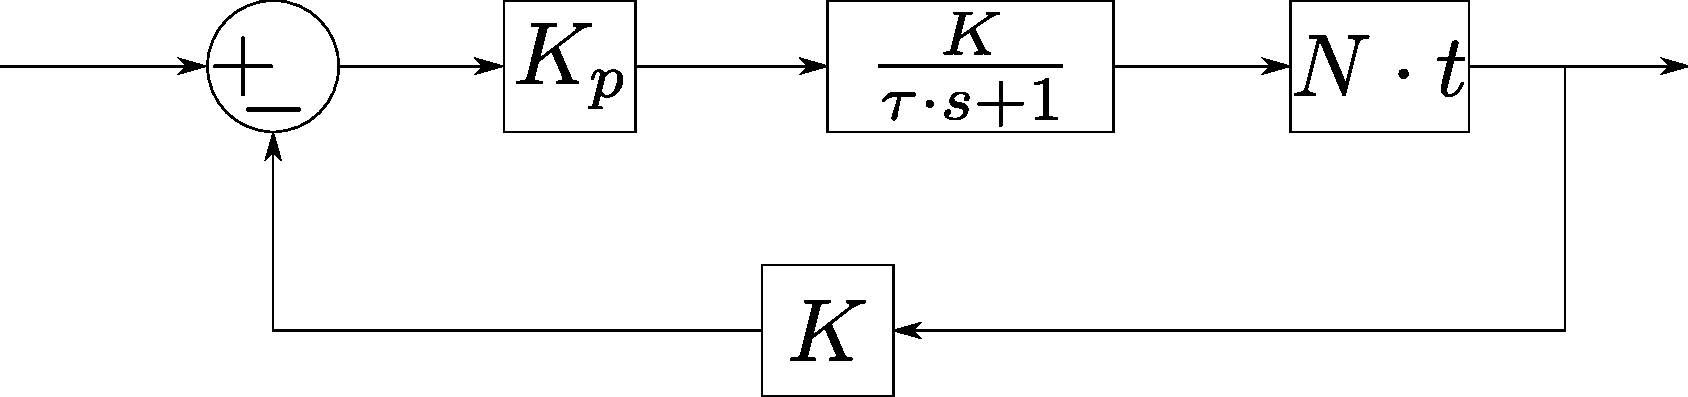
\includegraphics[scale=0.6]{figures/proportionalController.pdf}
 	\caption{Diagram of the proportional controller}
  \label{proportionalController}
\end{figure}

The illustrated diagram yields the following closed loop transfer function:
%
\begin{flalign}
  \eq{ \frac{V_{out}}{V_{ref}} }{\frac{\frac{K_p \cdot K}{\tau \cdot s +1}}{1 + \frac{K_p \cdot K}{\tau \cdot s +1}} = \frac{1}{ \frac{ \tau \cdot s + 1 }{ K_p \cdot K + 1 } + 1} = \frac{\frac{ K_p \cdot K }{ K_p \cdot K + 1 } }{ \frac{ \tau }{ K_p \cdot K + 1 } \cdot s + 1}}&
\label{eq:PclosedLoopTfs}
\end{flalign}
%
From \eqref{eq:PclosedLoopTfs} it is evident that the time constant and the gain for the system is dependent on the chosen \si{K_p}. The time constant of the closed loop transfer function is the coefficient of s in standard form:
%
\begin{flalign}
  \eq{ \tau_{closed} }{ \frac{ \tau }{ K_p \cdot K + 1 } }&\nonumber
\end{flalign}
%
As an example, the \si{K_p} is chosen such that it cancels out the gain, \si{K}, of the plant. This results in a time constant and a gain which is reduced to half:

\begin{flalign}
  \eq{ \frac{V_{out}}{V_{ref}} }{ \frac{\frac{ \frac{1}{K} \cdot K }{ \frac{1}{K} \cdot K + 1 } }{ \frac{ \tau }{ \frac{1}{K} \cdot K + 1 } \cdot s + 1} }&\nonumber\\
  \eq{ \frac{V_{out}}{V_{ref}} }{\frac{\frac{1}{2}}{\frac{\tau}{2} \cdot s + 1}}&\label{eq:PclosedLoop}
\end{flalign}
%
This results in the P-controller giving an output of half the input, but rise to its set-point twice as fast as the system step without control. This is tested utilizing the vehicle and the response is as expected. The test can be seen in \appref{app:proportionalControllerTest}.
%

If a system where an input velocity is equal to an output velocity is desired, a P-controller is insufficient. The reason lies in the numerator in \eqref{eq:PclosedLoopTfs}. No matter the value of \si{K_p} the numerator will always be less than 1. This results in an offset. A larger \si{K_p} resulting in a smaller offset, will make the coefficient of s in \eqref{eq:PclosedLoopTfs} (time constant) smaller, which can result in larger overshoot.

\subsection{P-Controller with Feed Forward}
The P-controllers difference between the reference and set-point, steady state offset, can be diminished without compromising the time constant, through use of feed forward, see \figref{proportionalControllerWithFeedforward}.
%
\begin{figure}[H]
 	\centering
 	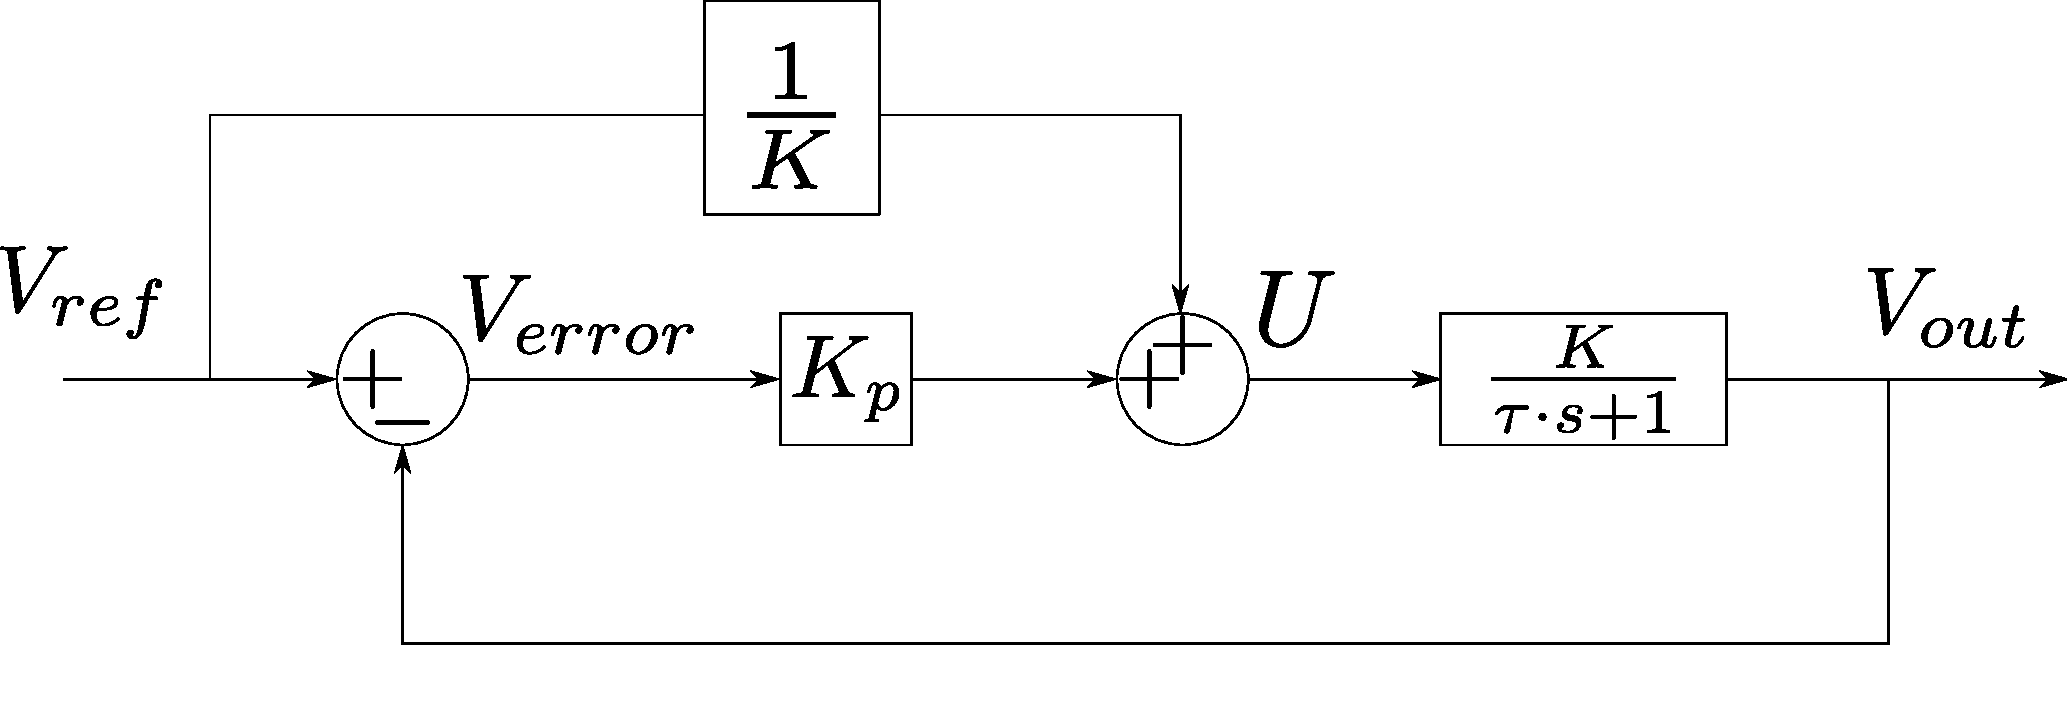
\includegraphics[scale=0.5]{figures/proportionalControllerWithFeedforward.pdf}
 	\caption{Diagram of the proportional controller with feedforward}
 	\label{proportionalControllerWithFeedforward}
\end{figure}
%
In this design the set-point is changed by feed forwarding the desired value of the output, \si{V_{out}}, to the input of the plant. Thereby summing up the desired value with the error, \si{V_e}, fed through the P-controller. The gain located on the feed forward ensures the input, \si{V_{ref}}, has the same unit as the signal going into the plant, in the case volts, \si{U}. Since the system gain, \si{K}, converts volts into linear velocity, the gain in the forward feed is set to \si{\frac{1}{K}}. The control loop in \figref{proportionalControllerWithFeedforward} yields the following closed loop transfer function:
%
\begin{flalign}
  \eq{ \frac{V_{out} }{V_{ref}} }{ \frac{\frac{K\cdot \frac{1}{K}+K\cdot K_p}{1+K \cdot K_p}}{\frac{\tau}{1+K\cdot K_p}\cdot s + 1 } }&\nonumber
\end{flalign}
%
If the \si{K_p} value is selected to cancel out the system gain, as with the P-controller, allowing for velocity directly on the controller input, the following equation emerges from the closed loop transfer function:
%
\begin{flalign}
  \eq{ \frac{V_{out} }{V_{ref}} }{ \frac{\frac{K\cdot \frac{1}{K}+K\cdot \frac{1}{K}}{1+K \cdot \frac{1}{K}}}{\frac{\tau}{1+K\cdot \frac{1}{K}}\cdot s + 1 } }&\nonumber\\
  \eq{ \frac{V_{out} }{V_{ref}} }{ \frac{1}{\frac{\tau}{2} \cdot s + 1} }&\nonumber
\end{flalign}
%
If this is compared to the resulting closed loop transfer function for the original P-controller, \eqref{eq:PclosedLoop}, it can be seen that the steady state offset is removed. Notice that the time constant of the closed loop remains half of that of the plant. 

By utilizing the feed forward to place the set-point of the controller, P-control becomes a viable option for controlling a velocity. This is tested utilizing the vehicle and the response is as expected. The test can be seen in \appref{app:proportionalControllerTest}. A Comparing of a step response utilizing the vehicle and a simulation of a step response is illustrated in figure \figref{fig:stepPfeedForward}.
%
\begin{figure}[H]
 	\centering
 	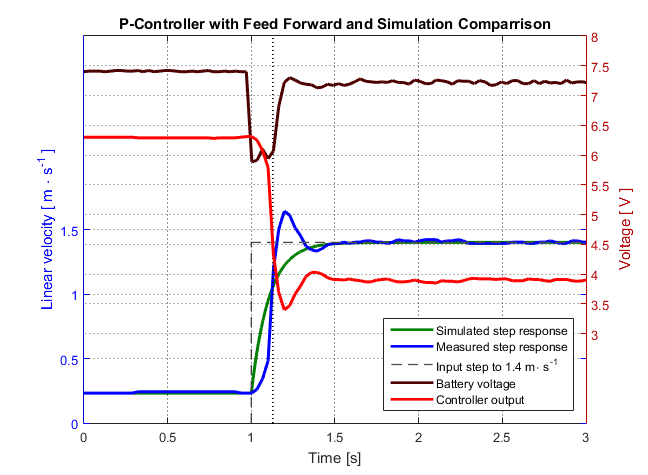
\includegraphics[width=.9\textwidth]{figures/stepPfeedForward}
 	\caption{Proportional control with feed forward. The simulation is first order while the vehicle is second order due to the armature coils in the motor.}
 	\label{fig:stepPfeedForward}
\end{figure}
%
There are a few things to notice. First, the rise time of the two are approximately equal, however, the simulation of the first order approximation rises directly, while the measured data has a delayed initial rise. This delay is presumably because of the armature coils in the motor, through which the current cannot change instantaneously. This effect gives rise to a second order term, as discussed in \secref{DriveTrain}, where the first order approximation was made. After the armature coils have been energized the controller output has a much faster effect on the velocity of the vehicle, causing it to rise so fast that it overshoots due to inertia.

An other interesting thing to notice is the sudden drop in battery voltage. When large currents are drawn from a NiMH battery, the voltage drops\cite{BatteryDS}. However in the implementation the duty cycle is scaled according to the current battery voltage, so that the controller maintains the same effect regardless of battery voltage. The exception being when the controller output exceeds the battery voltage, in which case the control will follow the battery voltage until the battery recovers. If the voltage drop at large current draws turn out to be a problem, an option could be to consider LiPO batteries, which are better at keeping a constant voltage, regardless of the amount of current drawn.
%
The P-controller with feed forward seems to be a good choice, however if subjected to disturbances some problems emerge. A disturbance imposed on the system is analogue to a sudden change of the gain of the plant. since the set-point compensation origins at the input of the controller, the sudden change in gain of the plant cannot be compensated for with this feed forward P-controller.
%
The effect is demonstrated in \figref{fig:hillPfeedForward}, where the feed forward controller is going up a hill.
%
\begin{figure}[H]
 	\centering
 	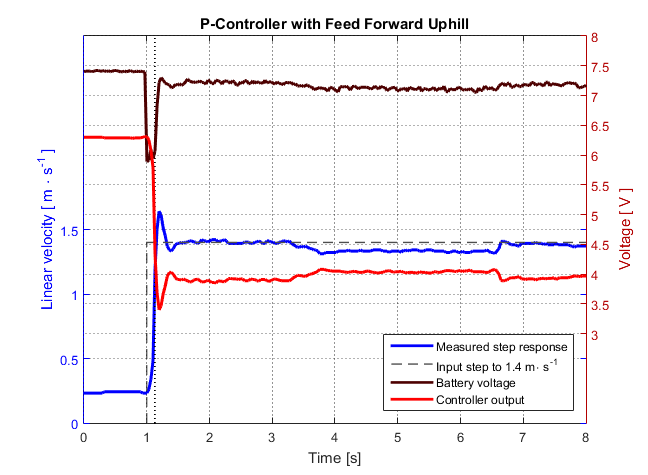
\includegraphics[width=.9\textwidth]{figures/hillPfeedForward}
 	\caption{When the P-controller with feed forward is subjected to constant disturbances, the gain of the system changes and the proportional gain and set-point is no longer sufficient, to avoid steady state error.}
 	\label{fig:hillPfeedForward}
\end{figure}
%
Since the vehicle steers by breaking on one side, this kind of steady state error will not only occur when encountering slopes, but every time the vehicle turns.
%
\subsection{PI-Controller} \label{sec:PIcalc}
To attack the new offset-problem caused by changes in the system gain when disturbances affects the system, a proportional integral controller is the next natural choice. The reason for choosing a PI-controller is because the I-component integrates over the error. This component therefore increases or decreases over time, and therefore has an adaptive effect on the system. The design is illustrated in \figref{proportionalIntegratorController}
%
\begin{figure}[H]
 	\centering
 	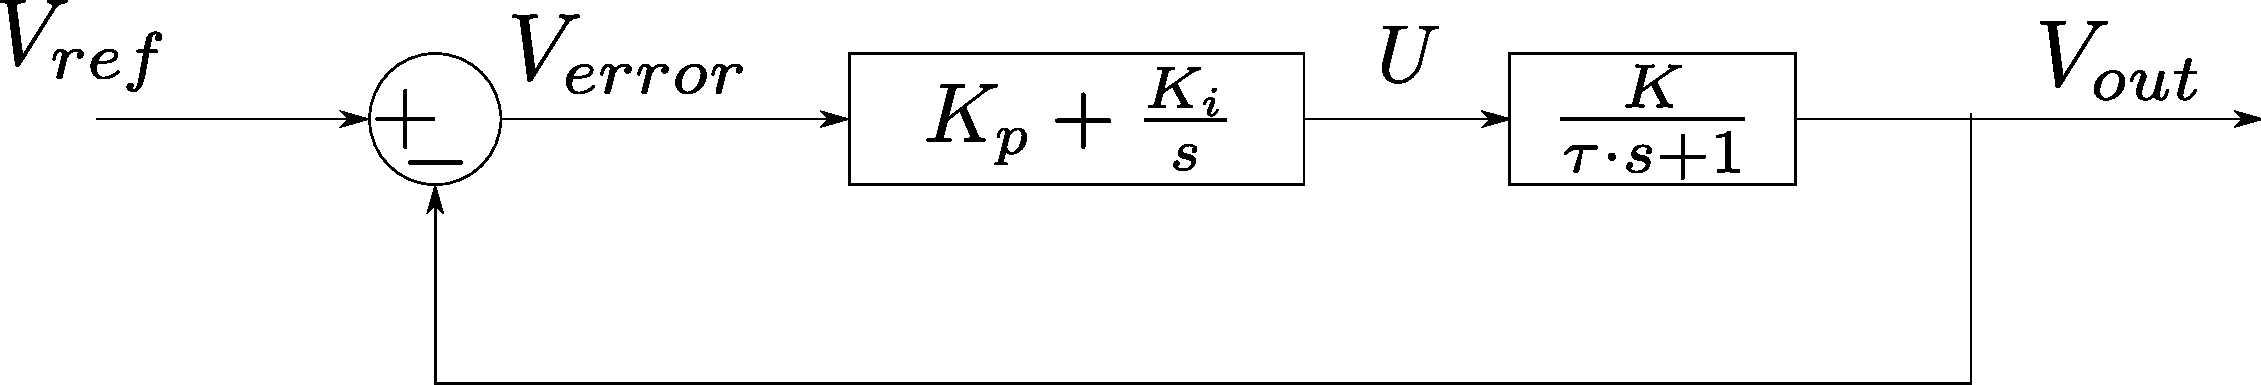
\includegraphics[scale=0.6]{figures/proportionalIntegratorController.pdf}
 	\caption{Diagram of the proportional integral controller}
 	\label{proportionalIntegratorController}
\end{figure}
%
The standard equation for a PI-controller can be rewritten to:
%
\begin{flalign}
  \eq{K_p\cdot\left(1+ \frac{1}{T_i\cdot s}\right)}{K_p \cdot \frac{T_i \cdot s + 1}{T_i \cdot s}}&\nonumber
\end{flalign}
%
Where \si{T_i} is the time constant of the integrator. Now if the time constant of the integrator is matched to the time constant of the plant, that is \si{T_i = \tau}, the following equation emerges from the closed loop transfer function:
%
\begin{flalign}
  \eq{\frac{V_{out} }{V_{ref}}}{\frac{K_p \cdot \frac{\tau \cdot s + 1}{\tau \cdot s} \cdot \frac{K}{\tau \cdot s + 1 }}{1 + K_p \cdot \frac{\tau \cdot s + 1}{\tau \cdot s} \cdot \frac{K}{\tau \cdot s + 1 }}}  \ \ \Leftrightarrow  \ \ 
  \si{\frac{V_{out} }{V_{ref}} = \frac{K_p \cdot \frac{K}{\tau \cdot s}}{1 + K_p \cdot \frac{K}{\tau \cdot s} }}&\nonumber
\end{flalign}
%
Inserting \si{K_p = \frac{1}{K}}, yields the following:
%
\begin{flalign}
  \eq{\frac{V_{out} }{V_{ref}}}{\frac{\frac{1}{K} \cdot \frac{K}{\tau \cdot s}}{1 + \frac{1}{K} \cdot \frac{K}{\tau \cdot s} }} \ \ \Leftrightarrow  \ \  \si{\frac{V_{out} }{V_{ref}} = \frac{\frac{1}{\tau \cdot s}}{1 + \frac{1}{\tau \cdot s} }} \ \ \Leftrightarrow  \ \  \si{\frac{V_{out} }{V_{ref}} = \frac{1}{\tau \cdot s + 1}}&\nonumber
 \label{eq:1overkinserted}
\end{flalign}
%
This is equivalent to the plant but with a gain of 1 instead of K, which is desirable, and so also the reason for inserting \si{K_p = \frac{1}{K}} in \eqref{eq:1overkinserted}.
Now to determine \si{K_i}, the original equation for a PI-controller is evaluated:
%
\begin{flalign}
  \si{K_p + K_i\cdot \frac{1}{s}} &= \si{K_p\cdot\left(1+ \frac{1}{T_i\cdot s}\right) \ \ \Rightarrow \ \ K_i\cdot \frac{1}{s} = \frac{K_p}{T_i\cdot s} \ \ \Rightarrow \ \ K_i = \frac{K_P}{T_i} \ \ \Rightarrow \ \ K_i = \frac{K_p}{\tau}}&\nonumber
\end{flalign}
%
This concludes the initial design of the PI-controller, however, in the following segment the controller will be analyzed and compared to the other controllers. Implementation and discussion of results follow immediately after.

\subsection{Comparison of the Controllers}
On \figref{fig:ControllerSteps} the different controller designs are simulated being subjected to a velocity step of 1.4 \si{m \cdot s^{-1}}. Furthermore, to compared the controllers with a step response of the plant, the plant is subjected to a voltage step calculated from the velocity step and the gain of the plant, corresponding to the value \si{K_p}. Since it is a step response of a plant, and not a controller, no feedback is utilized.
%
\begin{figure}[H]
 	\centering
 	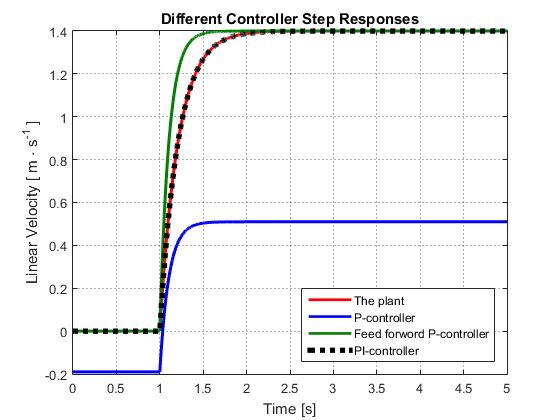
\includegraphics[width=.8\textwidth]{figures/ControllerSteps}
 	\caption{Diagram of the proportional controller}
 	\label{fig:ControllerSteps}
 \end{figure}
%
A thing to notice on \figref{fig:ControllerSteps}, is the inadequacy of the P-controller, given by its steady state error. The feed forward P-controller however, solving this problem, seems like a very good solution if consulting only its step response. As discussed, a problem arises when introducing a disturbance, as seen in \figref{fig:hillPfeedForward}. The last discussed option is the PI-controller, which places itself right on top of the step response of the plant when having a gain of 1, which is by design. The difference between the plant with a scaled input to obtain a gain of 1, compared to the PI-controller lies in the feedback along with the adaptive gain emerging from the I-component. It becomes clear when investigating the open loop rather than the closed loop transfer function:
%
\begin{flalign}
  V_{error}(s) \cdot \frac{(K_p \cdot \frac{K_i}{s}) \cdot K}{\tau \cdot s + 1}
  \left.\rule{0cm}{1cm}\right\vert\rule{0cm}{.7cm}_{\substack{K_p = \frac{1}{K} \\ \rule{0cm}{.1cm}\\ K_i = \frac{K_p}{\tau}}}
  &\ \ \Rightarrow \ \
  V_{error}(s) \cdot \frac{1}{\tau \cdot s}
  \ \ \xRightarrow{\mathcal{L^{\si{-1}}}} \ \
  \frac{1}{\tau} \cdot \int_{0}^{t} V_{error}(\tau_i) \ d \tau_i &\nonumber
\end{flalign}
%
\hspace{6mm} Where:\\
\begin{tabular}{p{1cm}lll}
  & \si{\tau_i}    & is an integration variable&\\
  & \si{V_{error}} & is the error from \si{V_{ref}-V_{out}}, see \figref{proportionalIntegratorController}&
\end{tabular}

This illustrates how the integral component, of the controller, integrates over the error from the reference to the output over time.

On \figref{fig:PIcontrollerStepRealVsSim} a step response of an implemented PI-controller and, to compare, a simulated step response the PI-controller, is illustrated.
%
\begin{figure}[H]
 	\centering
 	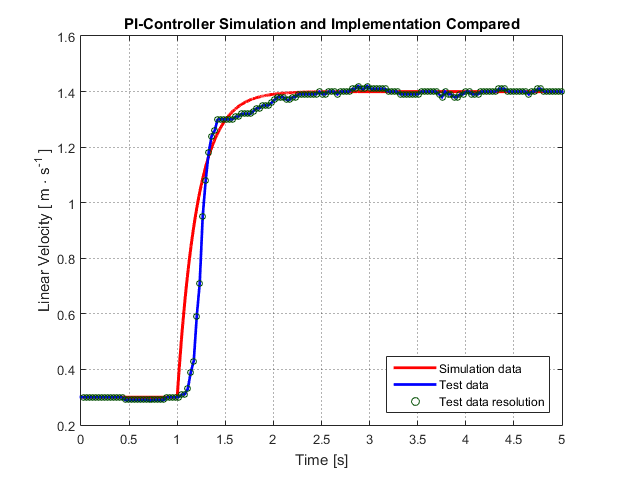
\includegraphics[width=.9\textwidth]{figures/PIcontrollerStepRealVsSim}
 	\caption{Diagram of the proportional integral controller compared to simulation}
 	\label{fig:PIcontrollerStepRealVsSim}
\end{figure}
%
The difference between the two responses at the bottom of the graph might, as mentioned for the feed forward P-controller, be partially due to the fact that the vehicle is a second order system. The approximation to a first order model is however not to be discarded. The design still delivers a response relatively close to the simulation.
If this implementation is investigated at different velocity steps, a certain characteristic of the current design can become more apparent, see \figref{fig:multiStepPI}.
%
\begin{figure}[H]
 	\centering
 	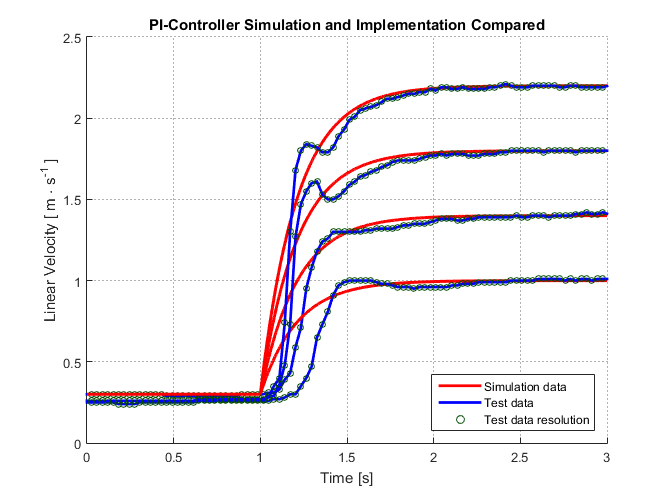
\includegraphics[width=.9\textwidth]{figures/multiStepPI}
 	\caption{Diagram of the proportional controller}
 	\label{fig:multiStepPI}
\end{figure}
%
The system overshoots before reaching the reference velocity. To investigate this behavior further a step is made at 2 \si{m\cdot s^{-1}}, and data from the battery and controller output is recorded, see \figref{fig:PInoAntiWindup}.
%
\begin{figure}[H]
 	\centering
 	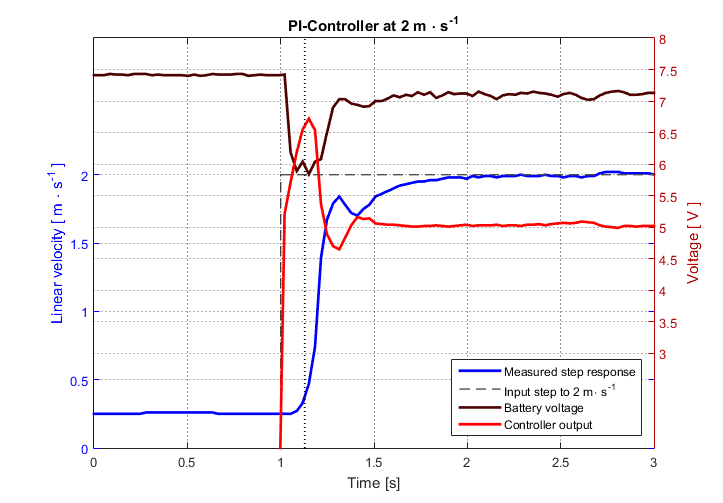
\includegraphics[width=.8\textwidth]{figures/PInoAntiWindup}
 	\caption{Diagram of the proportional controller}
 	\label{fig:PInoAntiWindup}
\end{figure}
%
As mentioned earlier, in this implementation the controller output is converted to duty cycle taking into account a varying battery voltage. So the battery voltage has an impact on the control only when the controller output exceeds the battery voltage. As a side note, the battery voltage is limited to a maximum of \si{100 \ \%} duty cycle.
The overshoot happens after the battery voltage saturation, and so the answer must be found elsewhere.

When the velocity of the vehicle rises, the error naturally falls, and the proportional error follows the error. The controller output follows this fall of the error, while the integral gain keeps building. This means that the controller output will keep falling until the integral gain takes over, which happens too late, compared to the settle value (5 V) of the controller output, causing it to overshoot. A smaller \si{K_p} would decrease the controller output overshoot by giving less gain in the rise, also increasing the time constant.
The delay from the overshoot of the controller to the velocity is caused by inertia in the system.
In the following section this overshoot will be further investigated.
%
\subsection{Implementation of the PI controller}
The functional part of the implementation is seen in \autoref{lst:PIimplementation}. The \emph{Actualspeed} is set from the average of recorded speeds of the two belts, from the Hall sensors. Then the error is calculated by comparison between the feedback, \emph{Actualspeed}, and the reference, \emph{Wantedspeed}.
A quick glance at \figref{fig:PInoAntiWindup}, reveals a problem, where the controller output exceeds the battery voltage. This is called empty integral windup, and can be prevented by implementing anti windup, which locks the integral error so that it does not make the controller output voltage exceed the saturation of the battery\todo{source here}. The first if-statement in \autoref{lst:PIimplementation}, is a very simple implementation of an anti-windup functionality, and the effect is clearly demonstrated by repeating the test from \figref{fig:PInoAntiWindup} with anti windup, as seen on figure \figref{fig:PIwithAntiWindup}.

%
\lstset{language=C++, caption={Implementation of the PI-controller}, label=lst:PIimplementation}
\begin{lstlisting}
Actualspeed = (speed0 + speed1)/2; // Average speed of the vehicle

Error = Wantedspeed - Actualspeed;                 //  ANTI-WINDUP:
                                                   //  Only increase integral error if
if( ControllerOutput < ((float)batReading/102.4) ) //<-the battery is not in saturation
{
  Integral = Integral + (Error*0.030); //Delta t = 0.03 s = sample time i.e. 30 ms
}

ControllerOutput = ((Kp * Error) + (Ki * Integral) + Stiction);

DutyPrSpeed = 100.0/((float)batReading/102.4); // Duty cycle pr volt [% pr V]
                                               // batReading/102.4 = volts
Duty = ControllerOutput * DutyPrSpeed;

if(Duty > 100) Duty = 100;  //maximum duty cycle = 100 %
if(Duty < 0) Duty = 0;      //minimum duty cycle =   0 %
\end{lstlisting}
%
\begin{figure}[H]
 	\centering
 	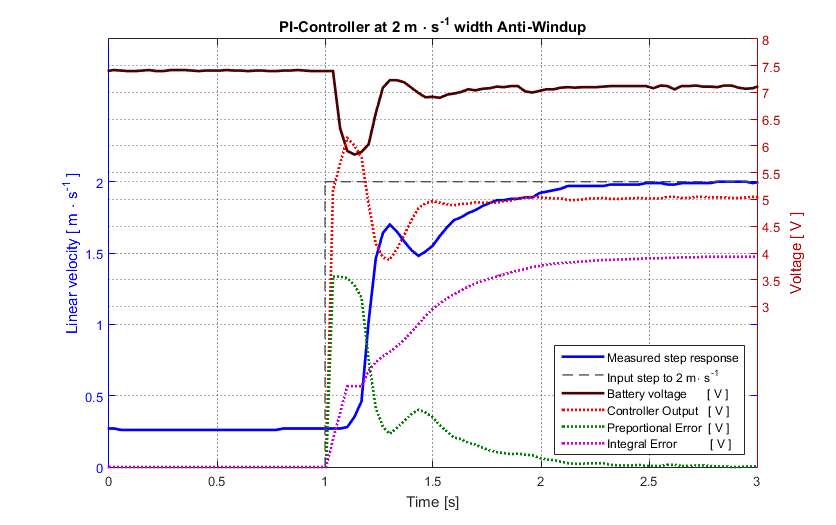
\includegraphics[width=.8\textwidth]{figures/PIwidthAntiWindup}
 	\caption{Diagram of the proportional controller}
 	\label{fig:PIwithAntiWindup}
\end{figure}
%
After making sure that the battery is not in saturation the integral error is increased or decreased depending on weather the error is positive or negative, see line 7 in \autoref{lst:PIimplementaion}. Finally in line 10 the \emph{ControllerOutput} is calculated, including the proportional gain, \si{K_p}, and the integral gain, \si{K_i}, along with the \emph{Stiction}, which is a voltage offset to counter the effect of stiction.
The duty cycle is then calculated in line 12 and 14, where it is scaled according to the current battery voltage, so that each controller output applies the calculated voltage, regardless of the battery voltage. This implementation with the calculated proportional and integral constants, see \secref{sec:PIcalc}, is tested at \si{1.4 m\cdot s^{-1}}, see \figref{fig:CalculatedPI}.
%
\begin{figure}[H]
 	\centering
 	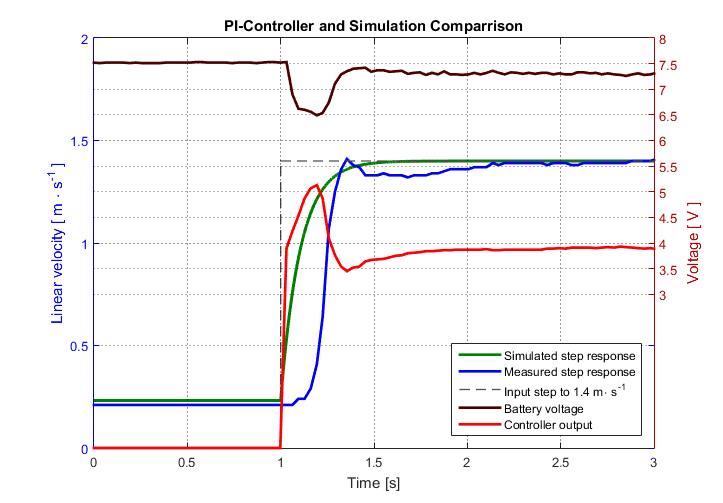
\includegraphics[width=.8\textwidth]{figures/CalculatedPI}
 	\caption{Diagram of the proportional controller}
 	\label{fig:CalculatedPI}
\end{figure}
%
The reality diverges from the simulation as previously mentioned, because it is a first order approximation. The previously addressed controller overshoot, can be minimized by tuning the proportional and integral gain, so that the transition between dominance of the two gains, becomes more smooth at the wanted operation speed, \si{1.4 m\cdot s^{-1}}. The tuning has been done with multiple iterations applying a trial and error approach. The result is shown on \figref{fig:TunedPI}, where the dip in the battery voltage is minimal, due to the longer rise-time, which also minimizes overshoot. 
%
\begin{figure}[H]
 	\centering
 	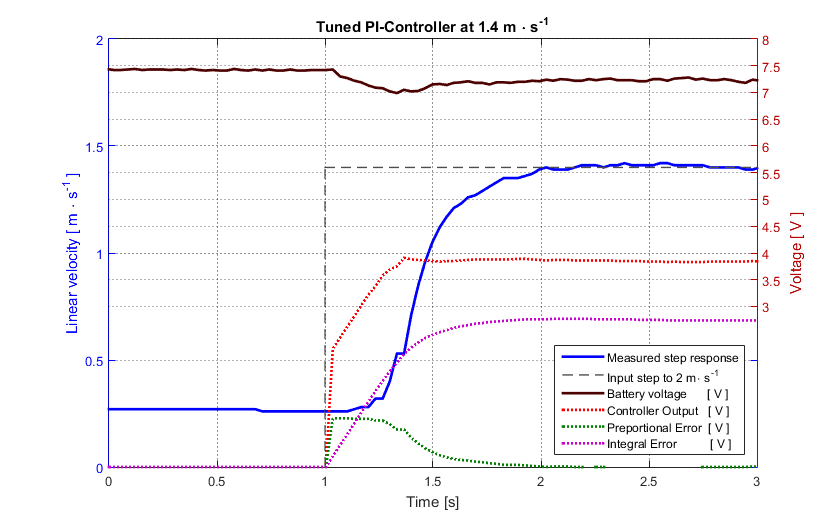
\includegraphics[width=.8\textwidth]{figures/TunedPI}
 	\caption{Diagram of the proportional controller}
 	\label{fig:TunedPI}
\end{figure}
%
The test is carried out on a ramp, which goes up and then flattens out. The same ramp was used for testing the P-controller with feed forward, see \figref{fig:hillPfeedForward}, where a steady state error occurred, while on the hill. Whereas the PI-controller's integral gain closes this steady state error, and so keeps the speed when on the hill.